\RequirePackage[l2tabu,orthodox]{nag} % for package advice

% TODO: decide if one-sided/two-sided
%\documentclass[headsepline,footsepline,footinclude=false,fontsize=11pt,paper=a4,listof=totoc,bibliography=totoc,BCOR=12mm,DIV=12]{scrbook} % two-sided
\documentclass[headsepline,footsepline,footinclude=false,oneside,fontsize=11pt,paper=a4,listof=totoc,bibliography=totoc]{scrbook} % one-sided

\PassOptionsToPackage{table,svgnames,dvipsnames}{xcolor}

% general/language
\usepackage[utf8]{inputenc}
\usepackage[T1]{fontenc}
\usepackage[sc]{mathpazo}
\usepackage[american]{babel}
\usepackage[autostyle]{csquotes}
\usepackage[%
  backend=bibtex,
  url=false,
  doi=false,
  style=numeric,
  giveninits,
  sorting=none,
  maxnames=10
]{biblatex}
\usepackage{booktabs} % for rulers in tables
\usepackage[final]{microtype} % for \microtypesetup{protrusion=true}
\usepackage[hidelinks, breaklinks = true]{hyperref} % hidelinks removes colored boxes around references and links, breaklinks allows linebreak in e.g. list of figures for long captions
%\usepackage[toc,nonumberlist,acronym]{glossaries} % TODO: remove if glossary not needed

% math
\usepackage{amsmath}
\usepackage{algorithm} %for algorithm environment
\usepackage{algpseudocode} %for algorithm environment
\usepackage{units} % for units
%\usepackage{scrhack} % necessary for listings package
%\usepackage{listings}

% graphics
\usepackage{graphicx}
\usepackage{psfrag}
\usepackage{epstopdf}
\usepackage{tikz}
\usepackage{lmodern}
\usepackage{pgf}
\usepackage{pgfplots}
\usepackage{pgfplotstable}

\usepackage{caption} % Required for custom captions
\usepackage{subcaption} % Required for subfigures


% Basic information for cover & title page
\newcommand*{\getUniversity}{Technical University of Munich} %{Technische Universität München}
\newcommand*{\getFaculty}{Department of Informatics}
\newcommand*{\getTitle}{Realistic Optimization-based Driving Using a Constrained Double-Integrator Model}
\newcommand*{\getTitleGer}{Realistisches, optimierungsbasiertes Fahren mit einem beschränkten Doppel Integrator Modell}
\newcommand*{\getAuthor}{Andreas Belavic}
\newcommand*{\getDoctype}{Bachelor's Thesis in Informatics}
\newcommand*{\getSupervisor}{Prof.
	Dr.-Ing.
	Matthias Althoff} \newcommand*{\getAdvisor}{M.Sc.
	Tobias Mascetta, M.Sc.
	Lukas Schäfer}
\newcommand*{\getSubmissionDate}{28.02.2025}
\newcommand*{\getSubmissionLocation}{Munich}

\newcommand{\arstretch}[1]{\renewcommand{\arraystretch}{#1}} %to change the row spacing in tables
% TODO: add custom commands etc.

% Settings for bibliography
\bibliography{content/literature}
% \addbibresource{content/literature}

% Settings for fonts
\setkomafont{disposition}{\normalfont\bfseries} % use serif font for headings
\linespread{1.05} % adjust line spread for mathpazo font

% Settings for glossaries
%\renewcommand{\glsnamefont}[1]{\normalfont\bfseries #1} % use serif font for glossary entry titles
%\makeglossaries{}

% Settings for pgfplots
\pgfplotsset{compat=1.9} % TODO: adjust to your installed version
\pgfplotsset{
	% For available color names, see http://www.latextemplates.com/svgnames-colors
	cycle list={CornflowerBlue\\Dandelion\\ForestGreen\\BrickRed\\},
}

% Settings for lstlistings
%\lstset{%
%  basicstyle=\ttfamily,
%  columns=fullflexible,
%  autogobble,
%  keywordstyle=\bfseries\color{MediumBlue},
%  stringstyle=\color{DarkGreen}
%}
% \newglossaryentry{computer}
{
  name=computer,
  description={is a machine that\ldots}
}
 % TODO: uncomment if glossary needed
% \newacronym{tum}{TUM}{Technische Universität München}
 % TODO: uncomment if list of abbreviations needed

\begin{document}
% \begin{titlepage}
  % HACK for two-sided documents: ignore binding correction for cover page.
  % Adapted from Markus Kohm's KOMA-Script titlepage=firstiscover handling.
  % See http://mirrors.ctan.org/macros/latex/contrib/koma-script/scrkernel-title.dtx,
  % \maketitle macro.
  \oddsidemargin=\evensidemargin\relax
  \textwidth=\dimexpr\paperwidth-2\evensidemargin-2in\relax
  \hsize=\textwidth\relax

  \centering

  \vspace{40mm}
  
\includegraphics[width=40mm]{./figures/tum}

  \vspace{5mm}
  {\LARGE \MakeUppercase{\getUniversity{}}}\\

  \vspace{5mm}
  {\Large \MakeUppercase{\getFaculty{}}}\\

  \vspace{20mm}
  {\Large \getDoctype{}}

  \vspace{15mm}
  {\huge\bfseries \getTitle{}}

  \vspace{15mm}
  {\LARGE \getAuthor{}}

  \vspace{20mm}
  %
\includegraphics[width=20mm]{logos/faculty}
	
\end{titlepage}


\frontmatter{}
% \begin{titlepage}
  \centering

  \vspace{40mm}
  
\includegraphics[width=40mm]{./figures/tum}

  \vspace{5mm}
  {\LARGE \MakeUppercase{\getUniversity{}}}\\

  \vspace{5mm}
  {\Large \MakeUppercase{\getFaculty{}}}\\

  \vspace{20mm}
  {\Large \getDoctype{}}

  \vspace{15mm}
  {\huge\bfseries \getTitle{}}

  \vspace{10mm}
  {\huge\bfseries \getTitleGer{}}

  \vspace{15mm}
  \begin{tabular}{l l}
    Author:          & \getAuthor{}         \\
    Supervisor:      & \getSupervisor{}     \\
    Advisor:         & \getAdvisor{}        \\
    Submission Date: & \getSubmissionDate{} \\
  \end{tabular}

  \vspace{20mm}
  %
\includegraphics[width=20mm]{logos/faculty}
\end{titlepage}

% \thispagestyle{empty}
\vspace*{0.65\textheight}
\noindent
I confirm that this bachelor's thesis is my own work and I have documented all sources and material used. \\\\
Ich versichere, dass ich diese Bachelor's Thesis selbständig verfasst und nur die angegebenen Quellen und Hilfsmittel verwendet habe.

\vspace{15mm}
\noindent
\getSubmissionLocation{}, \getSubmissionDate{} \hspace{5cm} \getAuthor{}

\cleardoublepage{}

% \addcontentsline{toc}{chapter}{Acknowledgments}
\thispagestyle{empty}

\vspace*{2cm}

\begin{center}
{\usekomafont{section} Acknowledgments}
\end{center}

\vspace{1cm}

A thesis may include an acknowledgments section where the author may want to thank certain people, groups, institutions, etc. who provided support.


\cleardoublepage{}

% \chapter{\abstractname}
This is the abstract.
It is a short summary of your work, consisting of roughly one to three paragraphs.
It should give the main ideas of your paper, i.e., the posed problem, a motivation for solving it, your solution method, and your results results
results.
Keep it understandable for a general audience.
Do not include references.

\microtypesetup{protrusion=false}
% \tableofcontents{}
\microtypesetup{protrusion=true}

\mainmatter{}
% \chapter{Introduction} \label{ch:intro}

The \textit{student starter kit} serves as guidance for students writing a thesis. This Latex document contains some advice on writing and can be used as template for your thesis. 
In addition, this starter kit contains a template for presentations, standardized grade sheets used to transparently mark your work, and a template for submitting your files (see Sec.~\ref{sec:submission}). As a short summary, the kit also contains two text files: a checklist for your thesis and one for your presentation; please adhere to them!

The student starter kit is only to be used within the Professorship Cyber-Physical Systems. The kit has been created by Markus Koschi\footnote{\href{mailto:markus.koschi@tum.de}{\texttt{markus.koschi@tum.de}}}. This latex template is based on the template by Florian Walch and contributors\footnote{\url{https://github.com/fwalch/tum-thesis-latex}}. The advice on format and style are from Carmella Schürmann. The advice on the literature review are from Matthias Althoff. 

Further reading is referenced where applicable, and general information provided by TUM is available in German\footnote{\url{https://www.tum.de/studium/studienabschluss/abschlussarbeit/tipps-und-tricks/}} and English\footnote{\url{https://www.tum.de/nc/en/studies/completing-your-studies/theses/tips-and-tricks/}}. The advice given by Elmar Juergens, a former PhD student at TUM in software engineering, might be also useful for you: \url{https://thesisguide.org/}.


\section{Submission} \label{sec:submission}
For internal archiving, you are required to submit all source files of your thesis, presentation, and software in the given format (see the enclosed submission folder):
The parent folder should be named firstNameLastName and contain the following sub-folders:
\begin{itemize}
\item papers\_FirstNameLastName (folder containing studied publications)
\item presentation\_FirstNameLastName (folder for the pdf and source files of the presentation)
\item report\_FirstNameLastName (folder for the pdf and source files of the report)
\item software\_FirstNameLastName (folder for the source files of the created software)
\end{itemize}
Please submit this folder at latest on the day of your presentation either via mail or personally by flash drive. The pdf of your thesis is required on the official day of submission. Note that you should aim at reproducible results, i.e., that your advisor can run your code and reproduce your results. Thus, providing a read-me and saving the simulation parameters in a script might be a good idea.

\section{Overview}
This document explains how to structure a thesis in Ch.~\ref{ch:format} and how to write well in Ch.~\ref{ch:Style}. Ch.~\ref{ch:latex} provides advice on how to use Latex, and Ch.~\ref{ch:lit_review} describes best practices to conduct a literature review.








\chapter{Single Track Model} \label{ch:sin_tra_mod}

\section{Model}

The state variables and control inputs for the single-track model are defined as follows:

\[
	x = \begin{bmatrix}
		s \\ n \\ \xi \\ v \\ \delta
	\end{bmatrix}
	\quad \text{(state variables)},
	\qquad
	u = \begin{bmatrix}
		a_{x,b} \\ v_\delta
	\end{bmatrix}
	\quad \text{(control inputs)}.
\]

,where the state consist of Frenet Frame Coordinates ($s$,$n$), a Heading Alignment Error $\xi$, a longitude vehicle velocity $v$ and a
steering angle $\delta$.
The state evolution is given by:

\[
	\dot{x} =
	\begin{bmatrix}
		\frac{v \cos\xi}{1 - nC(s)}                \\[8pt]
		v \sin\xi                                  \\[8pt]
		\frac{1}{l_{wb}}v \tan\delta - C(s)\dot{s} \\[8pt]
		a_{x,b}                                    \\[8pt]
		v_\delta
	\end{bmatrix}.
\]

\section{Assumptions}

To simplify the model, the following assumptions are made:

\begin{itemize}
	\item $C(s)$ is constant.
	\item $nC(s)$ is close to zero.
\end{itemize}

\section{Non-Linear Terms}

The following approximations are applied to linearize the model:

\begin{itemize}
	\item $\frac{v \cos\xi}{1 - nC(s)} \approx v \cos\xi \approx v$
	\item $v \sin\xi \approx v \xi$
	\item $v \tan\delta \approx v \delta$
\end{itemize}

\section{Handling Bilinear Terms}

To handle bilinear terms of the form \(w = xy\), the following constraints are applied based on the bounds of \(x\) and \(y\):

\[
	x^L \leq x \leq x^U, \qquad y^L \leq y \leq y^U.
\]

The resulting constraints for \(w\) are:

\[
	\begin{aligned}
		w & \geq x^L y + x y^L - x^L y^L, \\
		w & \geq x^U y + x y^U - x^U y^U, \\
		w & \leq x^U y + x y^L - x^U y^L, \\
		w & \leq x^L y + x y^U - x^L y^U.
	\end{aligned}
\]

\chapter{Derivation of the Integrator Model} \label{ch:der_int_mod}

\section{Assumptions}

1. External accelerations can be directly controlled:
\begin{equation}
	u = \begin{bmatrix} a_{x,b}, & a_{y,b}, & a_\psi \end{bmatrix}, \quad a_b = \begin{bmatrix} a_{x,b}, & a_{y,b} \end{bmatrix}
\end{equation}
\\
2. Orientation of the vehicle $\psi$ equals the angle of the road $\theta$:
\begin{equation}
	\xi = \psi - \theta = 0
\end{equation}
which implies:
\begin{itemize}
	\item $a_b = a_t$
	\item $\dot{\psi} = \dot{\theta} = \frac{d\theta}{ds} \cdot \frac{ds}{dt} = C(s)\dot{s}$
	\item $a_\psi = \ddot{\psi} = \ddot{\theta} = C'(s) \dot{s}^2 + C(s)\ddot{s}$
\end{itemize}
3. $C'(s) = C'$ is constant.

\section{Further Simplification}

1. Define artificial input variables:
\begin{equation}
	\tilde{u} :=
	\begin{bmatrix}
		u_t \\ u_n
	\end{bmatrix} =
	\begin{bmatrix}
		\frac{
			a_{x,tn} + 2\dot{n}C(s)\dot{s} + nC'(s)\dot{s}^2
		}{
			1 - nC(s)
		} \\
		a_{y,tn} - C(s)\dot{s}^2(1 - nC(s))
	\end{bmatrix}
\end{equation}

\section{Resulting Integrator Model}

State:
\[
	x_{tn} = \begin{bmatrix} s, & n, & \dot{s}, & \dot{n} \end{bmatrix}
\]
Input:
\[
	\tilde{u} = \begin{bmatrix} u_t, & u_n \end{bmatrix}
\]
The integrator model is given by:
\begin{equation}
	\dot{x}_{tn} = \begin{bmatrix}
		0 & 0 & 1 & 0 \\
		0 & 0 & 0 & 1 \\
		0 & 0 & 0 & 0 \\
		0 & 0 & 0 & 0 \\
	\end{bmatrix} x_{tn} + \begin{bmatrix}
		0 & 0 \\
		0 & 0 \\
		1 & 0 \\
		0 & 1 \\
	\end{bmatrix} \tilde{u}
\end{equation}

\section{Constraints}

The constraints are defined by:
\begin{align}
	g(x_{tn}, \tilde{u}) :=
	\begin{bmatrix}
		(1 - nC(s)) u_t - (2\dot{n}C(s)\dot{s} + nC' \dot{s}^2) \\
		u_n + C(s) \dot{s}^2 (1 - nC(s))
	\end{bmatrix}
\end{align}
\\
Define the constraint set $\mathcal{Z}$ as:
\begin{equation}
	\mathcal{Z} = \left\{
	\begin{bmatrix} x_{tn} \\ \tilde{u} \end{bmatrix} \; \middle|\;
	\begin{aligned}
		 & C_{min} \leq C(s) \leq C_{max},                                                                                                                                              \\
		 & n_{min} \leq n \leq n_{max},                                                                                                                                                 \\
		 & \begin{bmatrix} v_{xmin} \\ v_{ymin} \end{bmatrix} \leq \begin{bmatrix} \dot{s}(1 + nC(s)) \\ \dot{n} \end{bmatrix} \leq \begin{bmatrix} v_{ymax} \\ v_{xmax} \end{bmatrix}, \\
		 & \dot{\psi}_{min} \leq C(s) \dot{s} \leq \dot{\psi}_{max},                                                                                                                    \\
		 & a_{\psi,b,min} \leq C' \dot{s}^2 + C(s) u_t \leq a_{\psi,b,max},                                                                                                             \\
		 & a_{b,min} \leq g(x_{tn}, \tilde{u}) \leq a_{b,max},                                                                                                                          \\
		 & ||g(x_{tn}, \tilde{u})||^2 \leq \text{const}
	\end{aligned}
	\right\}
\end{equation}

\section{Constraint Approximation Problem}

Given $\mathcal{Z}$, find an inner approximation $\underline{\mathcal{Z}}$ of $\mathcal{Z}$ such that $\underline{\mathcal{Z}}$ can be described with a set of constraints following the Disciplined Convex Programming (DCP) rules:
\begin{itemize}
	\item affine $==$ affine
	\item convex $\leq$ concave
	\item concave $\geq$ convex
\end{itemize}

\section{\texorpdfstring{$\forall$}{For all}-Elimination}

For a constraint not following the DCP rules, of the form:
\begin{equation}
	c_{min} \leq f(x, y) \leq c_{max}
\end{equation}
with $x \in \mathbb{R}$, $y \in \mathbb{R}^n$, and $f: \mathbb{R}^{n+1} \to \mathbb{R}$, where $c_{min}, c_{max} \in \mathbb{R}$ are constants. Further, if $f$ is affine in $x$, represented by:
\begin{equation}
	f(x, y) = a(y) x + b(y)
\end{equation}
with $a, b : \mathbb{R}^n \to \mathbb{R}$, bounds on $a(y)$ and $b(y)$ can be chosen:
\[
	a_{min} \leq a(y) \leq a_{max}, \quad b_{min} \leq b(y) \leq b_{max}
\]
Thus, an inner approximation of the set $Z$ defined by $c_{min} \leq f(x, y) \leq c_{max}$ can be given by:
\begin{equation}
	\begin{aligned}
		 & \underline{Z} =                                                                                                                                                                    \\
		 & \left\{ x \in \mathbb{R} \;\middle|\; \forall y \in \mathbb{R}^n : a(y) \in [a_{min}, a_{max}] \land b(y) \in [b_{min}, b_{max}] \implies f(x, y) \in  [c_{min}, c_{max}] \right\} \\
		 & \times \left\{ y \in \mathbb{R}^n \;\middle|\; a(y) \in [a_{min}, a_{max}] \land b(y) \in [b_{min}, b_{max}] \right\}                                                              \\
		 & =: X \times Y
	\end{aligned}
\end{equation}
\subsection{Calculate \texorpdfstring{$X$}{X}}
\textbf{Assumptions:}
\begin{equation}
	c_{min} \leq b_{min} \text{ and } b_{max} \leq c_{max} \text{ (or } a(y) \neq 0 \text{ TODO)}
\end{equation}
\\
\textbf{Definitions:}
\begin{equation}
	x_{min} := \max \left\{ \min\left\{ 0, \frac{c_{min} - b_{min}}{a_{max}} \right\}, \min\left\{ 0, \frac{c_{max} - b_{max}}{a_{min}} \right\} \right\}
\end{equation}

\begin{equation}
	x_{max} := \min \left\{ \max\left\{ 0, \frac{c_{max} - b_{max}}{a_{max}} \right\}, \max\left\{ 0, \frac{c_{min} - b_{min}}{a_{min}} \right\} \right\}
\end{equation}
\\
\textbf{Claim:}
\begin{equation}\label{claim}
	X = [x_{min}, x_{max}]
\end{equation}
\\
\textbf{Sub-Claim:}
\begin{equation}
	x_{min} < 0 < x_{max}
\end{equation}
\\
\textbf{Proof of Claim \eqref{claim}:}

Let \( x \in X \).

\textbf{Case Distinction for \( x_{min} \):}

\begin{itemize}
	\item \textbf{Case 1:} \( x_{min} = \frac{c_{min} - b_{min}}{a_{max}} \)
	      \begin{equation}
		      a_{max} x_{min} + b_{min} = c_{min} \leq a_{max} x + b_{min} \implies x_{min} \leq x
	      \end{equation}

	\item \textbf{Case 2:} \( x_{min} = \frac{c_{max} - b_{max}}{a_{min}} \)
	      \begin{equation}
		      a_{min} x_{min} + b_{max} = c_{max} \geq a_{min} x + b_{max} \implies x_{min} \leq x
	      \end{equation}
\end{itemize}

\textbf{Case Distinction for \( x_{max} \):}

\begin{itemize}
	\item \textbf{Case 1:} \( x_{max} = \frac{c_{max} - b_{max}}{a_{max}} \)
	      \begin{equation}
		      a_{max} x_{max} + b_{max} = c_{max} \geq a_{max} x + b_{max} \implies x_{max} \geq x
	      \end{equation}

	\item \textbf{Case 2:} \( x_{max} = \frac{c_{min} - b_{min}}{a_{min}} \)
	      \begin{equation}
		      a_{min} x_{max} + b_{min} = c_{min} \leq a_{min} x + b_{min} \implies x_{max} \geq x
	      \end{equation}
\end{itemize}

Therefore, we have:
\begin{equation}
	x_{min} \leq x \leq x_{max}
\end{equation}

Let \( x \in [x_{min}, x_{max}] \), \( y \in Y \).

\textbf{Case Distinction for \( a(y) \):}

\begin{itemize}
	\item \textbf{Case 1:} \( a(y) > 0 \)
	      \begin{equation}
		      a(y) x + b(y) \leq a(y) x_{max} + b(y) \leq a_{max} \frac{c_{max} - b_{max}}{a_{max}} + b_{max} = c_{max}
	      \end{equation}
	      \begin{equation}
		      a(y) x + b(y) \geq a(y) x_{min} + b(y) \geq a_{max} \frac{c_{min} - b_{min}}{a_{max}} + b_{min} = c_{min}
	      \end{equation}

	\item \textbf{Case 2:} \( a(y) < 0 \)
	      \begin{equation}
		      a(y) x + b(y) \leq a(y) x_{min} + b(y) \leq a_{min} \frac{c_{max} - b_{max}}{a_{min}} + b_{max} = c_{max}
	      \end{equation}
	      \begin{equation}
		      a(y) x + b(y) \geq a(y) x_{max} + b(y) \geq a_{min} \frac{c_{min} - b_{min}}{a_{min}} + b_{min} = c_{min}
	      \end{equation}

	\item \textbf{Case 3:} \( a(y) = 0 \)
	      \begin{equation}
		      a(y) x + b(y) = b(y) \in [c_{min}, c_{max}]
	      \end{equation}
\end{itemize}

Therefore,
\begin{equation}
	\forall y \in Y: a(y) x + b(y) \in [c_{min}, c_{max}] \implies x \in X
\end{equation}

\subsection{Example}

Given $v_{_xmin}\leq \dot{s}(1 + nC(s)) \leq v_{_xmin}$.
\\
Set:
\begin{itemize}
	\item $x = \dot{s}$
	\item $y = \begin{bmatrix} n \\ C(s) \end{bmatrix}$
	\item $a(y) = 1 + y_1 y_2$
	\item $b(y) = 0$
\end{itemize}
Bounds for $a(y), b(y)$:
\begin{itemize}
	\item $a_{min} = 1 + \min \left\{ C_{min}n_{min}, C_{min}n_{max}, C_{max}n_{min}, C_{max}n_{max} \right\}$
	\item $a_{max} = 1 + \max \left\{ C_{min}n_{min}, C_{min}n_{max}, C_{max}n_{min}, C_{max}n_{max} \right\}$
	\item $b_{min} = b_{max} = 0$
\end{itemize}
One can now easily calculate $[x_{min}, x_{max}] = X$ and $Y$ can be expressed as $[C_{min}, C_{max}] \times [n_{min}, n_{max}]$
\chapter{Format} \label{ch:format}
This chapter introduces the basic layout of your thesis. In general, you want to make sure that each chapter flows smoothly and is linked to the one before. One way to do this is to briefly (in half a sentence or less) summarize what was discussed in the previous chapter, though you do not want to become too repetitive. If this cannot be done well, then leave it out. More critical is a short overview of what your reader can expect in the current chapter. Consider the possibility that your reader may not only read your work from start to finish in one go, but may also re-read certain chapters individually or out-of-order. 

\begin{itemize}
	\item \textit{In the previous chapter, xyz was discussed. Now we turn to.../Now we will look at.../In this chapter...}
\end{itemize}

What follows is a general outline, although there is no one ``correct'' way to format your thesis. The sections given in this reference guide (Introduction, Approach, Evaluation, etc.) each refer to a different chapter of your thesis. The subsections presented here correlate therefore to chapter sections. Depending on what makes sense for your topic and how you formulate your argument, certain parts can be merged or split. As mentioned above, make sure to tell a complete story from beginning to end, i.e., structure each chapter as a mini-thesis with an introduction, main part, and conclusion (though not necessarily divided that way into sections). For more information, see e.g. this website\footnote{\url{https://student.unsw.edu.au/thesis-structure}}.


\section{Introduction} \label{sec:intro}
The first chapter of your text. Clearly state your problem, what your work attempts to do, as well as why it is important. This should be understandable for a general audience, as you do not know who will be reading your thesis. 

Present the related work. Explain what has already been accomplished/solved -- and then explain what your approach offers that previous ones do not. What are their disadvantages, and how does your approach improve upon their drawbacks? The literature review section should summarize and evaluate related works, thus proving to your reader that your presented problem exists. To find related work, see the advise presented in Ch.~\ref{ch:lit_review}.

Once you have presented the previous approaches, restate your approach, its novelty, and the methods you use. Present the challenges of your approach as well -- you are not going to save all the world's problems with your thesis, but you can try to make it easier to do so. Do not make sweeping claims and over-generalizations, e.g., \textit{This topic is the most important of this generation and many to come.}

End the introduction with an outline of your paper. Introduce each chapter/section and give a brief summary of what they contain. \textit{This paper/thesis/work is structured as follows: In Chapter 2...is presented in Chapter 3....Chapter 4 discusses...}

Often, it is useful to write the introduction after you have completed the rest of the paper: that way, you can correctly summarize what you set out to accomplish in the first place and how you did so. However, you should review related work as soon as you start your thesis to not reinvent the wheel.


\section{Approach}
This can be considered the main part of your work. Here, you want to go into detail about your approach. Explain the concept and methods used, as well as any shortcomings it may have. 

\subsection{Implementation/Method}
Depending on your approach, a description of your implementation may merit its own section or subsection. If the approach you are presenting is more general and/or can be applied to different areas, you may only have the time and resources for one example implementation.

This section should therefore describe your implementation process throughly and precisely, giving all necessary parameters, so that your reader can reproduce your results. If necessary, your source code can go in the appendix. 


\section{Numerical Experiments}
Here, you should give the results of your implementation and critically discuss them in detail. In order to prove the applicability/relevancy of your thesis, you typically also need to compare your approach to others. You should clearly define the setup and parameters of your experiment, then give your results and discuss them in detail. If your results are unexpected, figure out why and explain that to the reader. 


\section{Conclusion}
Here is the place to summarize what you have written: your goal, your approach, your results. Discuss what can be drawn from what you have achieved. End the thesis by describing your future work, i.e., what from your approach can be expanded and improved upon in further projects.
\chapter{Style} \label{ch:Style}
This chapter provides some information and tips about writing style.
As TUM student, you can benefit from free consulting of the English Writing
Center\footnote{\url{https://www.sprachenzentrum.tum.de/sprachen/englisch/english-writing-center/}}, which are highly recommended so that your
scientific advisor can focus her/his support on the content of your work (rather than having to polish language first).

\section{General Information}
Keep it simple.
Your reader should be able to reach the end of a sentence and remember how it began.
If your sentences are long and complicated, see if you can break them up.

\section{Punctuation}
English punctuation can be tricky.
Many rules are steadfast -- there are no exceptions.
Others, however, vary based on which style manual one uses.
In general, there are two preferred styles for technical fields like computer science: that of the \textbf{Institute of Electrical Engineers (IEEE)}
and that of the \textbf{Association for Computing Machinery (ACM)}.
You can find more information about their citation formatting on their respective websites or in Section \ref{sec:Citation}.
The \textbf{IEEE} style falls under the broader Chicago Manual of Style, so the answers to punctuation and syntax questions can be found there.
Note that these all use American formatting standards.

\subsection{Commas}
Some typical rules regarding commas include:
\begin{enumerate}
	\item You \textbf{must} put a comma between two \textbf{independent clauses} (i.e., complete sentences) which are joined by a conjunction, \textit{for, and, nor, but, or, yet, so}.
	      \begin{itemize}
		      \item The exception to this rule is very short sentences -- \textit{I computed A and my partner computed B}.
		            It is unlikely that you will encounter such sentences in your writing, so this exception can be ignored 95\% of the time.
	      \end{itemize}
	\item To avoid confusion, use the serial/Oxford comma, i.e., the final comma in a list with three or more items.
	      %\item You \textbf{may} omit the final comma in a list with three or more items; \textbf{however}, IEEE (and by extension, Chicago) Style typically requires the use of the serial/Oxford comma.
	      \begin{itemize}
		      \item For example: We present our method, our results, and a discussion.
	      \end{itemize}
	      %	\begin{itemize}
	      %		\item My \$ 10 million estate is to be split among my husband, daughter, son, and nephew.
	      %	\end{itemize}
	      %	Omitting the comma after son would indicate that the son and nephew would have to split one-third of the estate.
	\item Never put a comma between \textit{to be} and \textit{that}.
	      Likewise, do not put a comma before any form of \textit{to be}.
	      \begin{itemize}
		      \item Incorrect: The biggest confusion, is that there is not enough data. \\
		            Incorrect: The biggest confusion is, that there is not enough data.\\
		            Correct: The biggest confusion is that there is not enough data.
	      \end{itemize}
	      *There may be instances when you \textit{should} put a comma before a form of \textit{to be}, but this will serve a different grammatical function, e.g., to set off an appositive.
	      An appositive is a noun or pronoun which is set next to another noun or pronoun in order to explain it.
	      For example: ``The conclusion, the part of the paper which summarizes everything, is the trickiest part to write.
	      ''
	\item Put a comma before ``which'' if the text that comes before it can be understood without the text that comes after it.
	      Otherwise, do not.
	      \begin{itemize}
		      \item For example: We use the xyz control method, which was presented in Chapter 2.
		            \begin{itemize}
			            \item Here, the fact that this method was presented in Chapter 2 is additional information.
			                  You can understand the sentence without it.
		            \end{itemize}
		            We use the control method which was presented in Chapter 2.
		            \begin{itemize}
			            \item Here, you need to define which control method you are referring to; thus, that information is vital to properly understanding the sentence.
		            \end{itemize}
	      \end{itemize}
	\item Ue a comma when beginning sentences with introductory words such as ``well'', ``now'', or ``yes''.
	\item According to the IEEE guidelines, you should put a comma after ``\textbf{i.e.}'' and ``\textbf{e.g.}'' This is widely accepted by most American style guides.
	      It is less common in British English.
	\item For more comma rules, see the enclosed document \texttt{more\_comma\_rules.pdf}.
\end{enumerate}

\subsection{Semi-Colon}
The semi-colon has two main functions.
It can be used to join two complete sentences whose meanings are closely related: ``The results are inconclusive; this is due to the fact that the
data does not represent all possibilities.
''

Additionally, the semi-colon can be used as a sort of ``super-comma'' when lists have internal punctuation: ``This section has an introduction, which
gives an overview; a main part, where the methods are discussed; and a conclusion.
''

\section{Parts of Speech - Common Errors}
In this section, common errors/confusing rules will be discussed.
\subsection{Adverbs}
What is an adverb, again?
An adverb modifies a verb, an adjective, another adverb, or even a phrase.
It typically, although not always, ends in ``-ly.
''

\subsubsection{Placement}
\underline{Modifying Adjectives}\\

\noindent When adverbs modify an adjective, they should be placed directly before the word they are modifying.
For example, ``\textit{Table 2 shows \textbf{similarly promising} results.
}''\\

\noindent \underline{Modifying Sentences}\\

\noindent When modifying sentences, adverbs can be placed in four different positions:
\begin{itemize}
	\item at the beginning: \textit{\textbf{Usually}, such experiments are doomed to fail from the start.}
	\item at the end: \textit{We then repeat these steps \textbf{frequently}.}\\
	      Adverbs appearing at the end of the sentence include:

	      \begin{itemize}
		      \item adverbs of frequency - \textit{usually}, \textit{normally}, \textit{often}, etc.
		      \item adverbs of manner, i.e., how - \textit{slowly}, \textit{badly}
		      \item adverbs of time - \textit{today}, \textit{this year}
	      \end{itemize}
	\item after \textit{to be} and auxiliary verbs, e.g., \textit{can}, \textit{may}, \textit{will}, etc.: \textit{The problem will \textbf{definitely} be fixed.}
	\item before all other verbs: \textit{We \textbf{quickly} solve the equation.}
\end{itemize}

\subsection{Verbs}
\subsubsection{Tense}
The question of tense can be rather complicated.
You may have learned that one should always use the present tense, even when referring to past literature.
Different styles have different rules, though often these ``rules'' are simply suggestions.
The main body of your text should be written in the present tense.
However, your literature review may use different tenses, depending on what you wish to express.

The generally accepted guidelines on using tenses in the literature review are as follows:
\begin{itemize}
	\item Simple Past: Use the simple past tense (\textit{found}, \textit{reported}, \textit{introduced}) when you are describing the results/methods of an already published paper.
	      This tense is used when the citation/source is the subject of the sentence: ``Smith [1] found that this method was not very successful.
	      ''
	\item Present: Use the present tense in the literature review if you are offering your own opinion of the literature.
	      For example, ``Smith [1] argues that this approach does not make sense; however, it is clear that the methodology had some flaws.
	      ''
	\item Present Perfect: This is typically used to indicate that the research you are citing is still ongoing/relevant, or that your source is quite recent It can also be used to generalize about past literature. - ``Similar findings have been discussed more recently [7], [8], [10].''
\end{itemize}

\subsubsection{Voice}
As with tense, selecting which voice (active or passive) has advocates in both corners.
Some writers will tell you to avoid the passive voice at all costs.
Others will say that scientific writing uses the passive voice much more often than other disciplines.
Overusing the passive voice can get dry though, so it is generally good to vary your sentences.

\begin{itemize}
	\item Active Voice:
	      \begin{itemize}
		      \item ``We show the results in Table 6.''
		      \item ``We then compute the following equation: ...''
	      \end{itemize}
	\item Passive Voice:
	      \begin{itemize}
		      \item ``The results are shown in Table 6.''
		      \item ``The following equation is then computed: ...''
	      \end{itemize}
\end{itemize}

\subsection{Person}
Do not use the first person singular (``I'') in an academic paper.
Instead, use ``we'' or use the passive voice.

\section{Regional Differences}
Unless otherwise stated, you are free to choose between American and British English.
Once you have done so, stay consistent and stick to the chosen style.
Set your spell-check accordingly.
Typical spelling differences between American and British English include:

\begin{itemize}
	\item ``o'' vs. ``ou'': \textit{behavior} (Am.) vs. \textit{behaviour} (Br.)
	\item ``er'' vs. ``re'': \textit{center} (Am.) vs. \textit{centre} (Br.)
	\item ``z'' vs. ``s'': \textit{analyzed} (Am.) vs. \textit{analysed} (Br.)
	\item double consonants: \textit{modeled, modeling} (Am.) vs. \textit{modelled, modelling} (Br.)
\end{itemize}

Reliable dictionaries are Merriam Webster\footnote{https://www.merriam-webster.com} (American) and the Oxford English
Dictionary\footnote{https://en.oxforddictionaries.com} (British).

\chapter{Latex} \label{ch:latex}
After learning about the content of a thesis, we will discuss how to present content using Latex. If you are familiar with Latex, you can skip this chapter; others will serve this as a time-saving starting point.


\section{Using this Template} \label{sec:Using_this_template}
This template is for your reference only. You do not have to adhere to this format and can change anything you like.

To use this template, configure some settings in the settings folder. Then, add your content in the content folder (you can use multiple \texttt{.tex} files, but it might be easier to only use one) and your references to \texttt{literature.bib} (see also Section \ref{sec:Citation}).

You can compile a pdf from \texttt{main.tex} either using \emph{pdflatex} or  \emph{latex + dvips + ps2pdf} (often configured as quick build). In an editor, e.g. Texmaker, you can set \texttt{main.tex} as master document, and thus compile from any file.


\section{Figures} \label{sec:Figures}
Figures are a very important tool to present content. A (good) visualization often helps the reader to understand your concepts. But do not forget to also explain in words what can be seen in the figure.

If you use \emph{pdflatex}, you can include \texttt{pdf} figures, and if you use \texttt{latex}, you can include \texttt{eps} figures (please always use vector graphics). To draw figures or edit plots you generate with MATLAB or Python, you can use Inkscape\footnote{\url{https://inkscape.org/en/}}.

Fig.~\ref{fig:scenario1} demonstrates how we include a figure. If you use \emph{latex + dvips + ps2pdf}, the \texttt{eps} is included and \emph{psfrag} replaces the letters \emph{a}, \emph{b}, and \emph{c} with latex code. If you use \emph{pdflatex}, you can save a \texttt{pdf} figure from Inkscape with the option to omit text in the pdf and create an additional \texttt{pdf\_tex} file, whose text will then be typeset with Latex (not shown here).

\begin{figure}[!htpb]
\centering
	\footnotesize
	\psfrag{a}[r][c]{Obstacle~1}	
	\psfrag{b}[l][c]{Obstacle~2}
	\psfrag{c}[c][c]{Obstacle~3}
	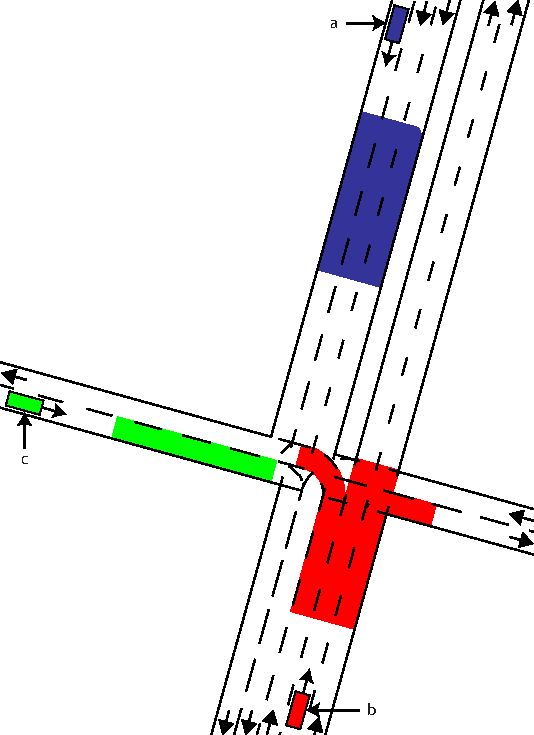
\includegraphics[width=0.4\columnwidth]{./figures/Scenario_Intersection_Occ_1,5-2,0s_final}
\caption{Occupancies of Obstacles~1, 2, and 3 in Scenario~I. The plot shows the initial configuration at $t_{0}$ and the predicted occupancies $\mathcal{O}(t)$ for ${t \in [t_{3}, t_{4}]}$.}
\label{fig:scenario1}
\end{figure}

\section{Math}
As an example, let us introduce $\mathcal{X}\subset\mathbb{R}^n$ as the set of feasible states $x$ and $\mathcal{U}\subset\mathbb{R}^m$ as the set of admissible control inputs $u$ of a system $f$, which is governed by the differential equation
\begin{equation}
	\begin{split}
	\dot{x}(t) &= f\big(x(t),u(t)\big). %\\
%	y&=g(x(t))
	\end{split}
	\label{eq:system}
\end{equation}

We assume that the initial time is $t_0 = 0$ and adhere to the notation $u([0, t_h])$ to describe a trajectory $u(t)\in\mathcal{U}$ for $t\in [0,t_h]$, $0<t_h$. Furthermore, $\chi\big(t_h,x(0),u([0,t_h])\big)\in\mathcal{X}$ denotes the solution of \eqref{eq:system} at time $t_h$ subject to $x(0)=x_0$ and $u([0,t_h])$.

Note that you should not reference an equation before introducing it. After giving the equation, you can refer to it, e.g., our system \eqref{eq:system} is awesome.


\section{Tables}
Tab.~\ref{tab:parameters} is an example of a nice table.

\begin{table}[!htb]\centering
\caption{Obstacle Parameters.}
\arstretch{1.3} 
\begin{tabular}{@{}llll@{}} \toprule
\textbf{Parameter} & \textbf{Variable} & \textbf{Parameter} &  \textbf{Variable} \\ \midrule
max. acceleration & $a_\mathrm{max}$ in $\unitfrac{m}{s^2}$ & Boolean for $C_\mathrm{back}$ & $b_\mathrm{back}$ \\ 
max. velocity & $v_\mathrm{max}$ in $\unitfrac{m}{s}$ & Boolean for $C_\mathrm{lane}$ & $b_\mathrm{lane}$ \\
switching velocity & $v_S$ in $\unitfrac{m}{s}$ & length & $l$ in $\unit{m}$ \\
speeding factor & $f_S$ & width & $w$ in $\unit{m}$ \\
\bottomrule
\end{tabular}
\label{tab:parameters}
\end{table}


\section{Algorithms}
Often, it will be helpful to describe your software by presenting pseudo code and explaining it (at least the significant lines). 

Alg.~\ref{alg:mainAlgorithm} shows the overall algorithm of \textit{SPOT}, which predicts the occupancy for a traffic participant up to the prediction horizon and can run in parallel for each traffic participant. First, the constraint management configures the parameters according to the set of last-measured states of the obstacle (line~\ref{alg:main_constraints}) as detailed in the next paragraph...

\begin{algorithm}
	\caption{Occupancy Prediction for an Obstacle}
	\begin{algorithmic}[1]
	\Require map
	\State parameters $\gets$ \Call{manageConstraints}{} \label{alg:main_constraints}
	\State reachableLanes $\gets$ \Call{reach}{map, parameters} \label{alg:main_reach}
	\ForAll{\Call{validAbstractions}{parameters}}
		\State $\mathcal{O}_{j}$ $\gets$ \Call{occupancy$_{j}$}{reachableLanes, parameters}\label{alg:main_abstractions}
	\EndFor
	\State \Return $\mathcal{O}$ $\gets$ \Call{intersect}{$\mathcal{O}_{j}$} \label{alg:main_intersect}
	\end{algorithmic}
	\label{alg:mainAlgorithm}
\end{algorithm}


\section{Citation} \label{sec:Citation}
For citations, we use a consecutively numbered citation style: bla \cite{latex} bla \cite{Koschi2017a, Althoff2017a} bla \cite{Paden2016}. To generate a bibliography file (the \texttt{.bib} file located in the folder content), you can use JabRef\footnote{\url{http://www.jabref.org/}}. Then, you run \textit{bibtex} and afterwards latex/pdflatex twice (as described in Sec.~\ref{sec:Using_this_template}).
\chapter{Literature Review} \label{ch:lit_review}

To find relevant works, you should follow this guideline:
\begin{itemize}
\item Important catalogues: IEEE XPlore, Google scholar, Scopus, Web of Science, Research Gate
\item Start searching catalogues: Write down used keywords and used catalogues to avoid repeating a search; try some searches with the keyword ``survey'' or ``overview'' to find survey papers
\item Group results: Find categories in which to put your found papers
\item Rank papers in each category: consider reputation of journal/conference, reputation of authors, and citations 
\item In best ranked papers: Look into their literature lists; what other papers are relevant (do this iteratively)? Newer papers are more useful since they cover the literture up to a later point in time. Finding a great and recent survey paper is the jackpot
\item Once the search has converged: identify the most important groups
\item Visit websites of important groups to identify missed papers
\end{itemize}

\appendix{}
%\microtypesetup{protrusion=false}
% \glsaddall{} % add all defined terms to glossary, even if not referenced in text
% \printglossaries{} % TODO: uncomment if glossary needed
\listoffigures{}
\listoftables{}
\printbibliography{}

\end{document}